\documentclass{ximera}
\graphicspath{  %% When looking for images,
{./}            %% look here first,
{./pictures/}   %% then look for a pictures folder,
{../pictures/}  %% which may be a directory up.
{../../pictures/}  %% which may be a directory up.
{../../../pictures/}  %% which may be a directory up.
{../../../../pictures/}  %% which may be a directory up.
}

\usepackage{listings}
\usepackage{circuitikz}
\usepackage{xcolor}
\usepackage{amsmath,amsthm}
\usepackage{subcaption}
\usepackage{graphicx}
\usepackage{tikz}
\usepackage{tikz-3dplot}
\usepackage{amsfonts}
\usepackage{mdframed} % For framing content
\usepackage{tikz-cd}

  \renewcommand{\vector}[1]{\left\langle #1\right\rangle}
  \newcommand{\arrowvec}[1]{{\overset{\rightharpoonup}{#1}}}
  \newcommand{\ro}{\texttt{R}}%% row operation
  \newcommand{\dotp}{\bullet}%% dot product
  \renewcommand{\l}{\ell}
  \let\defaultAnswerFormat\answerFormatBoxed
  \usetikzlibrary{calc,bending}
  \tikzset{>=stealth}
  




%make a maroon color
\definecolor{maroon}{RGB}{128,0,0}
%make a dark blue color
\definecolor{darkblue}{RGB}{0,0,139}
%define the color fourier0 to be the maroon color
\definecolor{fourier0}{RGB}{128,0,0}
%define the color fourier1 to be the dark blue color
\definecolor{fourier1}{RGB}{0,0,139}
%define the color fourier 1t to be the light blue color
\definecolor{fourier1t}{RGB}{173,216,230}
%define the color fourier2 to be the dark green color
\definecolor{fourier2}{RGB}{0,100,0}
%define teh color fourier2t to be the light green color
\definecolor{fourier2t}{RGB}{144,238,144}
%define the color fourier3 to be the dark purple color
\definecolor{fourier3}{RGB}{128,0,128}
%define the color fourier3t to be the light purple color
\definecolor{fourier3t}{RGB}{221,160,221}
%define the color fourier0t to be the red color
\definecolor{fourier0t}{RGB}{255,0,0}
%define the color fourier4 to be the orange color
\definecolor{fourier4}{RGB}{255,165,0}
%define the color fourier4t to be the darker orange color
\definecolor{fourier4t}{RGB}{255,215,0}
%define the color fourier5 to be the yellow color
\definecolor{fourier5}{RGB}{255,255,0}
%define the color fourier5t to be the darker yellow color
\definecolor{fourier5t}{RGB}{255,255,100}
%define the color fourier6 to be the green color
\definecolor{fourier6}{RGB}{0,128,0}
%define the color fourier6t to be the darker green color
\definecolor{fourier6t}{RGB}{0,255,0}

%New commands for this doc for errors in copying
\newcommand{\eigenvar}{\lambda}
%\newcommand{\vect}[1]{\mathbf{#1}}
\renewcommand{\th}{^{\text{th}}}
\newcommand{\st}{^{\text{st}}}
\newcommand{\nd}{^{\text{nd}}}
\newcommand{\rd}{^{\text{rd}}}
\newcommand{\paren}[1]{\left(#1\right)}
\newcommand{\abs}[1]{\left|#1\right|}
\newcommand{\R}{\mathbb{R}}
\newcommand{\C}{\mathbb{C}}
\newcommand{\Hilb}{\mathbb{H}}
\newcommand{\qq}[1]{\text{#1}}
\newcommand{\Z}{\mathbb{Z}}
\newcommand{\N}{\mathbb{N}}
\newcommand{\q}[1]{\text{``#1''}}
%\newcommand{\mat}[1]{\begin{bmatrix}#1\end{bmatrix}}
\newcommand{\rref}{\text{reduced row echelon form}}
\newcommand{\ef}{\text{echelon form}}
\newcommand{\ohm}{\Omega}
\newcommand{\volt}{\text{V}}
\newcommand{\amp}{\text{A}}
\newcommand{\Seq}{\textbf{Seq}}
\newcommand{\Poly}{\textbf{P}}
\renewcommand{\quad}{\text{    }}
\newcommand{\roweq}{\simeq}
\newcommand{\rowop}{\simeq}
\newcommand{\rowswap}{\leftrightarrow}
\newcommand{\Mat}{\textbf{M}}
\newcommand{\Func}{\textbf{Func}}
\newcommand{\Hw}{\textbf{Hamming weight}}
\newcommand{\Hd}{\textbf{Hamming distance}}
\newcommand{\rank}{\text{rank}}
\newcommand{\longvect}[1]{\overrightarrow{#1}}
% Define the circled command
\newcommand{\circled}[1]{%
  \tikz[baseline=(char.base)]{
    \node[shape=circle,draw,inner sep=2pt,red,fill=red!20,text=black] (char) {#1};}%
}

% Define custom command \strikeh that just puts red text on the 2nd argument
\newcommand{\strikeh}[2]{\textcolor{red}{#2}}

% Define custom command \strikev that just puts red text on the 2nd argument
\newcommand{\strikev}[2]{\textcolor{red}{#2}}

%more new commands for this doc for errors in copying
\newcommand{\SI}{\text{SI}}
\newcommand{\kg}{\text{kg}}
\newcommand{\m}{\text{m}}
\newcommand{\s}{\text{s}}
\newcommand{\norm}[1]{\left\|#1\right\|}
\newcommand{\col}{\text{col}}
\newcommand{\sspan}{\text{span}}
\newcommand{\proj}{\text{proj}}
\newcommand{\set}[1]{\left\{#1\right\}}
\newcommand{\degC}{^\circ\text{C}}
\newcommand{\centroid}[1]{\overline{#1}}
\newcommand{\dotprod}{\boldsymbol{\cdot}}
%\newcommand{\coord}[1]{\begin{bmatrix}#1\end{bmatrix}}
\newcommand{\iprod}[1]{\langle #1 \rangle}
\newcommand{\adjoint}{^{*}}
\newcommand{\conjugate}[1]{\overline{#1}}
\newcommand{\eigenvarA}{\lambda}
\newcommand{\eigenvarB}{\mu}
\newcommand{\orth}{\perp}
\newcommand{\bigbracket}[1]{\left[#1\right]}
\newcommand{\textiff}{\text{ if and only if }}
\newcommand{\adj}{\text{adj}}
\newcommand{\ijth}{\emph{ij}^\text{th}}
\newcommand{\minor}[2]{M_{#2}}
\newcommand{\cofactor}{\text{C}}
\newcommand{\shift}{\textbf{shift}}
\newcommand{\startmat}[1]{
  \left[\begin{array}{#1}
}
\newcommand{\stopmat}{\end{array}\right]}
%a command to give a name to explorations and hints and theorems
\newcommand{\name}[1]{\begin{centering}\textbf{#1}\end{centering}}
\newcommand{\vect}[1]{\vec{#1}}
\newcommand{\dfn}[1]{\textbf{#1}}
\newcommand{\transpose}{\mathsf{T}}
\newcommand{\mtlb}[2][black]{\texttt{\textcolor{#1}{#2}}}
\newcommand{\RR}{\mathbb{R}} % Real numbers
\newcommand{\id}{\text{id}}

\author{Zack Reed}
%borrowed from selinger linear algebra
\title{Learning Activity: }
\begin{document}
\begin{abstract}

    In this learning activity, you will be 
\end{abstract}
\maketitle


    \section*{Orthogonal Projections}

     
    Given a line $l$ and a vector $\vec{v}$ emanating from a point on $l$, it is sometimes convenient to express $\vec{v}$ as the sum of a vector $\vec{v}_{\parallel}$, parallel to $l$, and a vector $\vec{v}_{\perp}$, perpendicular to $l$.  If you have taken a physics course, you may have seen a force vector decomposed into the sum of two components: one parallel and one perpendicular to the direction of motion.
     
    \begin{center}
     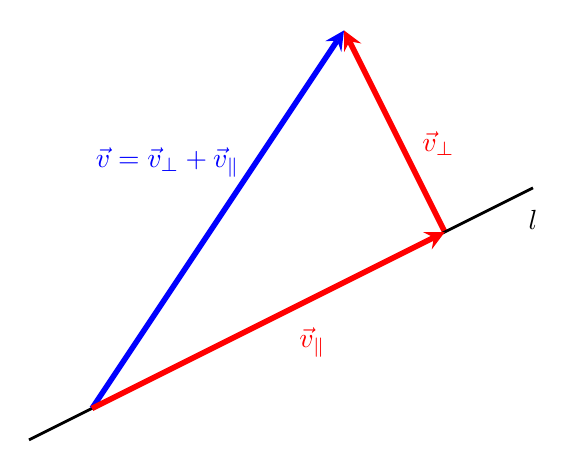
\begin{tikzpicture}[scale=.8]
      \draw[line width=2pt,red,-stealth](3.6, 0.8)--(2,4);
      \node[red] at (3.5, 2.2)   (a) {$\vec{v}_{\perp}$};
     \node[red] at (1.5, -0.95)   (b) {$\vec{v}_{\parallel}$};
      \node[] at (5, 1)   (c) {$l$};
      \node[blue] at (-0.8, 1.9)   (d) {$\vec{v}=\vec{v}_{\perp}+\vec{v}_{\parallel}$};
       \draw [-,line width=1pt]  (-3,-2.5)--(5, 1.5);
    \draw[line width=2pt,blue,-stealth](-2, -2)--(2,4);
    \draw[line width=2pt,red,-stealth](-2, -2)--(3.6, 0.8);
    \end{tikzpicture}
     
    \end{center}
     
    Suppose $\vec{d}$ is a direction vector for $l$.  Then $\vec{v}_
    {\parallel}=k\vec{d}$ for some scalar $k$.  Our goal is to find $k$. 
    \begin{align*}\vec{v}\dotp\vec{d}&=(\vec{v}_{\parallel}+\vec{v}_{\perp})\dotp\vec{d}\\
    &=(k\vec{d}+\vec{v}_{\perp})\dotp\vec{d}\\
    &=k\vec{d}\dotp\vec{d}+\vec{v}_{\perp}\dotp\vec{d}\\
    &=k\norm{\vec{d}}^2+0\\
    &=k\norm{\vec{d}}^2
    \end{align*}
    We conclude that $$k=\frac{\vec{v}\dotp\vec{d}}{\norm{\vec{d}}^2}$$
    and $$\vec{v}_{\parallel}=k\vec{d}=\left(\frac{\vec{v}\dotp\vec{d}}{\norm{\vec{d}}^2}\right)\vec{d}$$
     
    The vector $\vec{v}_{\parallel}=\left(\frac{\vec{v}\dotp\vec{d}}{\norm{\vec{d}}^2}\right)\vec{d}$ is called the \dfn{projection of $\vec{v}$ onto $\vec{d}$}.  In our discussion, $\vec{d}$ is a direction vector for line $l$.  So, we can also say that $\vec{v}_{\parallel}$ is the \dfn{projection of $\vec{v}$ onto $l$}.
     
    To find $\vec{v}_{\perp}$, observe that $\vec{v}_{\perp}=\vec{v}-\vec{v}_{\parallel}$.
     
     
    \begin{definition}\label{def:projection}
    Let $\vec{v}$ be a vector, and let $\vec{d}$ be a non-zero vector.  The \dfn{projection of $\vec{v}$ onto $\vec{d}$} is given by
    $$\mbox{proj}_{\vec{d}}\vec{v}=\left(\frac{\vec{v}\dotp\vec{d}}{\norm{\vec{d}}^2}\right)\vec{d}$$
    \end{definition}
     
    \begin{example}\label{ex:projection1}
    Find the projection of $\vec{v}$, shown below, onto the line given by $y=\frac{1}{2}x-1$.
     
    \begin{center}
    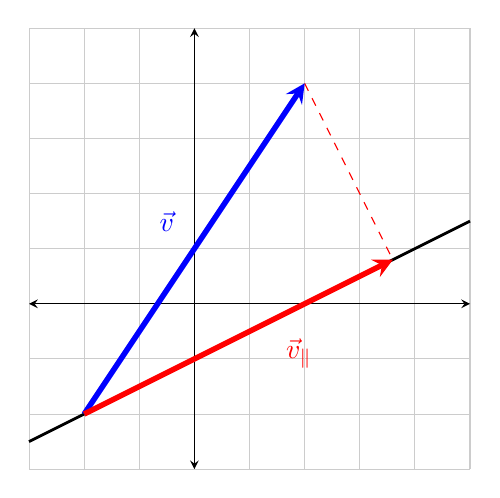
\begin{tikzpicture}[scale=.7]
     
    \draw[thin,gray!40] (-3,-3) grid (5,5);
      \draw[<->] (-3,0)--(5,0);
      \draw[<->] (0,-3)--(0,5);
      \draw[red, dashed] (2,4)--(3.6, 0.8);
      \draw [-,line width=1pt]  (-3,-2.5)--(5, 1.5);
    \draw[line width=2pt,blue,-stealth](-2, -2)--(2,4);
    \draw[line width=2pt,red,-stealth](-2, -2)--(3.6, 0.8);
    \node[blue] at (-0.5, 1.5)   (a) {$\vec{v}$};
    \node[red] at (1.9, -0.9)   (b) {$\vec{v}_{\parallel}$};
    \end{tikzpicture}
    \end{center}
     
    \begin{explanation}
    We begin by finding vectors $\vec{v}$ and $\vec{d}$. The tail of $\vec{v}$ is located at $(-2, -2)$, and the head of $\vec{v}$ is at $(2, 4)$.  Using the ``head-tail" formula we get
    $$\vec{v}=\begin{bmatrix}2-(-2)\\4-(-2)\end{bmatrix}=\begin{bmatrix}4\\6\end{bmatrix}$$ The direction vector for the line $y=\frac{1}{2}x-1$ is $$\vec{d}=\begin{bmatrix}2\\1\end{bmatrix}$$
    We find that $\vec{v}\dotp\vec{d}=14$ and $\norm{\vec{d}}^2=5$.
    Thus $$\mbox{proj}_{\vec{d}}\vec{v}=\left(\frac{\vec{v}\dotp\vec{d}}{\norm{\vec{d}}^2}\right)\vec{d}=\frac{14}{5}\begin{bmatrix}2\\1\end{bmatrix}=\begin{bmatrix}28/5\\14/5\end{bmatrix}$$
    \end{explanation}
    \end{example}
     
    \subsection*{Distance from a Point to a Line}
     
    The shortest distance from a point to a line is the length of the perpendicular line segment dropped from the point to the line.  Vector projection formula will help us find the length of such a perpendicular.
     
    \begin{example}\label{ex:distancefrompttoline}
    Let $A(2, -1, 1)$ be a point in $\RR^3$.  Suppose line $l$ is given by parametric equations $$x=t+3$$
    $$y=-t+1$$
    $$z=t-2$$
     
    \begin{center}
    \begin{tikzpicture}[scale=.6]
       
       \draw [-,line width=1pt]  (-3,-2.5)--(5, 1.5);
       \node[] at (5, 0.8)   (a) {$l$};
    \fill (2, 4)node[above, right]{$A(2, -1, 1)$} circle (1mm);
    \end{tikzpicture}
    \end{center}
     
    Find the distance from $A$ to $l$.
    \begin{explanation}
    We will first construct a vector $\vec{v}$ by picking an arbitrary point $B$ on $l$ to be the tail of $\vec{v}$ and using point $A$ as the head of $\vec{v}$.  An easy point to choose on line $l$ is the point $(3, 1, -2)$ that corresponds to $t=0$.  Now we have
    $$\vec{v}=\overrightarrow{BA}=\begin{bmatrix}2-3\\-1-1\\1-(-2)\end{bmatrix}=\begin{bmatrix}-1\\-2\\3\end{bmatrix}$$
     
    \begin{center}
    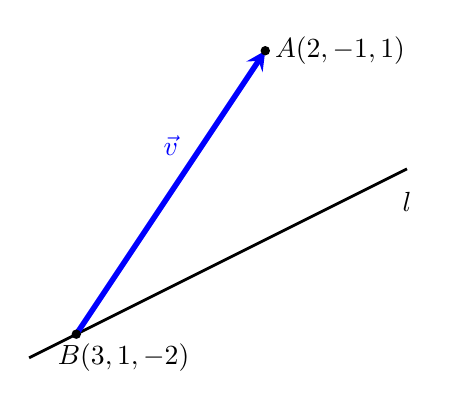
\begin{tikzpicture}[scale=.6]
       
       \draw [-,line width=1pt]  (-3,-2.5)--(5, 1.5);
        \node[] at (5, 0.8)   (a) {$l$};
    \draw[line width=2pt,blue,-stealth](-2, -2)--(2,4);
     
    \fill (-2, -2) circle (1mm);
    \fill (2, 4)node[below, right]{$A(2, -1, 1)$} circle (1mm);
    \node[] at (-1, -2.5)   (b) {$B(3, 1, -2)$};
    \node[blue] at (0, 2)   (c) {$\vec{v}$};
    \end{tikzpicture}
    \end{center}
     
    The line has a direction vector
    $$\vec{d}=\begin{bmatrix}1\\-1\\1\end{bmatrix}$$
     
    We will now find the projection of $\overrightarrow{BA}$ onto $l$  $$\mbox{proj}_{\vec{d}} \overrightarrow{BA}=\left(\frac{\vec{v}\dotp\vec{d}}{\norm{\vec{d}}^2}\right)\vec{d}=\frac{4}{3}\begin{bmatrix}1\\-1\\1\end{bmatrix}=\begin{bmatrix}4/3\\-4/3\\4/3\end{bmatrix}$$
     
    \begin{center}
    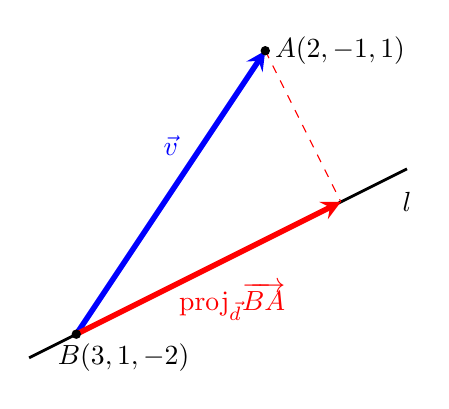
\begin{tikzpicture}[scale=.6]
       
       \draw [-,line width=1pt]  (-3,-2.5)--(5, 1.5);
       \node[] at (5, 0.8)   (a) {$l$};
       \node[] at (-1, -2.5)   (b) {$B(3, 1, -2)$};
    \node[blue] at (0, 2)   (c) {$\vec{v}$};
    \node[red] at (1.3, -1.3)   (d) {$\mbox{proj}_{\vec{d}}\overrightarrow{BA}$};
    \draw[line width=2pt,blue,-stealth](-2, -2)--(2,4);
    \draw[line width=2pt,red,-stealth](-2, -2)--(3.6, 0.8);
    \draw[red, dashed] (2,4)--(3.6, 0.8);
    \fill (-2, -2)  circle (1mm);
    \fill (2, 4)node[above, right]{$A(2, -1, 1)$} circle (1mm);
    \end{tikzpicture}
    \end{center}
     
     
    Next, we find $\vec{v}_{\perp}$.
    $$\vec{v}_{\perp}=\vec{v}-\vec{v}_{\parallel}=\begin{bmatrix}-1\\-2\\3\end{bmatrix}-\begin{bmatrix}4/3\\-4/3\\4/3\end{bmatrix}=\begin{bmatrix}-7/3\\-2/3\\5/3\end{bmatrix}$$
     
    \begin{center}
    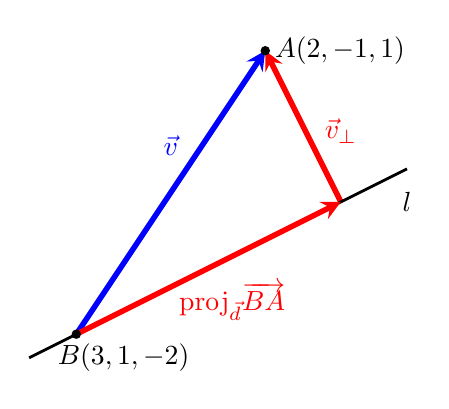
\begin{tikzpicture}[scale=.6]
      \draw[line width=2pt,red,-stealth](3.6, 0.8)--(2,4);
       \draw [-,line width=1pt]  (-3,-2.5)--(5, 1.5);
       \node[] at (5, 0.8)   (a) {$l$};
       \node[] at (-1, -2.5)   (b) {$B(3, 1, -2)$};
    \node[blue] at (0, 2)   (c) {$\vec{v}$};
    \node[red] at (1.3, -1.3)   (d)
    {$\mbox{proj}_{\vec{d}}\overrightarrow{BA}$};
    \node[red] at (3.6, 2.3)   (e) {$\vec{v}_{\perp}$};
    \draw[line width=2pt,blue,-stealth](-2, -2)--(2,4);
    \draw[line width=2pt,red,-stealth](-2, -2)--(3.6, 0.8);
    \fill (-2, -2)  circle (1mm);
    \fill (2, 4)node[above, right]{$A(2, -1, 1)$} circle (1mm);
    \end{tikzpicture}
    \end{center}
     
     
    Finally, to find the distance between point $A$ and line $l$, we find the magnitude of $\vec{v}_{\perp}$.
    $$\norm{\vec{v}_{\perp}}=\frac{1}{3}\sqrt{49+4+25}=\frac{\sqrt{78}}{3}$$
    \end{explanation}
    \end{example}
     
    \section*{Practice Problems}
    \emph{Problems \ref{prob:proj1a}-\ref{prob:proj1b}}
     
    Find $\mbox{proj}_{\vec{d}}\vec{v}$. 
     
      \begin{problem}\label{prob:proj1a}
      If $\vec{d}=\begin{bmatrix}-1\\3\end{bmatrix}$ and $\vec{v}=\begin{bmatrix}1\\4\end{bmatrix}$ then
      $$\mbox{proj}_{\vec{d}}\vec{v}=\begin{bmatrix}\answer{-1.1}\\\answer{3.3}\end{bmatrix}$$
        \end{problem}
         
        \begin{problem}\label{prob:proj1b}
        If $\vec{d}=\begin{bmatrix}0\\2\\1\end{bmatrix}$ and $\vec{v}=\begin{bmatrix}-1\\-4\\2\end{bmatrix}$ then
        $$\mbox{proj}_{\vec{d}}\vec{v}=\begin{bmatrix}\answer{0}\\\answer{-2.4}\\\answer{-1.2}\end{bmatrix}$$
        \end{problem}
     
    \begin{problem}\label{prob:proj2}
    Find the projection of vector $\vec{v}$ onto line $l$. (If entering answers in decimal form, round to the nearest one hundredth.)
     
    \begin{center}
    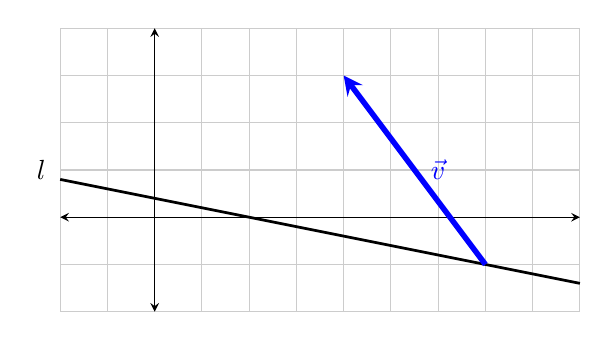
\begin{tikzpicture}[scale=.6]
    \draw[thin,gray!40] (-2,-2) grid (9,4);
      \draw[<->] (-2,0)--(9,0);
      \draw[<->] (0,-2)--(0,4);
      \node[blue] at (6, 1)   (a) {$\vec{v}$};
      \node[] at (-2.4, 1)   (b) {$l$};
      \draw [-,line width=1pt]  (-2,0.8)--(9, -1.4);
    \draw[line width=2pt,blue,-stealth](7, -1)--(4,3);
    \end{tikzpicture}
    \end{center}
     
    Answer:
    $$\begin{bmatrix}\answer[tolerance=0.005]{-95/26}\\\answer[tolerance=0.005]{19/26}\end{bmatrix}$$
    \end{problem}
     
    \begin{problem}\label{prob:distpttoline}
    Find the distance between point $A$ and line $l$.
     
    \begin{center}
    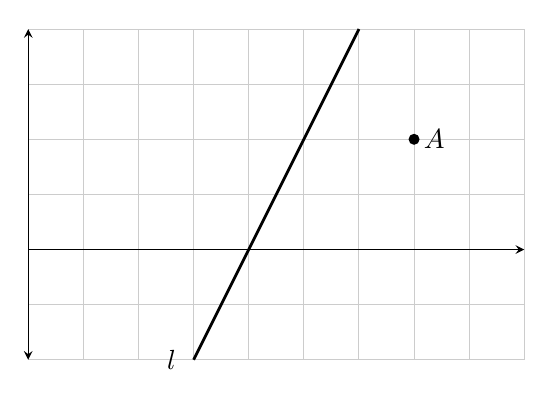
\begin{tikzpicture}[scale=.7]
    \draw[thin,gray!40] (0,-2) grid (9,4);
      \draw[->] (0,0)--(9,0);
      \draw[<->] (0,-2)--(0,4);
      \fill (7,2)node[above, right]{$A$} circle (1mm);
      \node[] at (2.6, -2)   (b) {$l$};
      \draw [-,line width=1pt]  (3,-2)--(6, 4);
    \end{tikzpicture}
    \end{center}
     
    Answer: $\sqrt{\answer{3.2}}$.
    \end{problem}
     
    \begin{problem}\label{prob:proj3}
    Show that $\mbox{proj}_{\vec{d}}\vec{v}$ does not depend on the length of $\vec{d}$ by proving that $\mbox{proj}_{\vec{d}}\vec{v}=\mbox{proj}_{k\vec{d}}\vec{v}$ for $k\neq 0$.  What does this result mean geometrically?  Illustrate your response with a diagram.
    \end{problem}
     
    \begin{problem}\label{prob:circletangenttoline}
    Find the radius of a circle centered at $(4, 2)$ if the line $y=\frac{3}{2}x+3$ is tangent to the circle.  Enter your response as a fraction.
     
    Answer:
    $$r=\sqrt{\answer{196/13}}$$
    The graph below shows the line $y=\frac{3}{2}x+3$ together with a circle of radius $1$.  Change the value of $r$ to the radius you have found to visualize the correct answer.
     
    \pdfOnly{
    Access GeoGebra interactives through the online version of this text at
     
    \href{https://ximera.osu.edu/oerlinalg}{https://ximera.osu.edu/oerlinalg}.
    }
     
    \begin{onlineOnly}
    \begin{center}
    \geogebra{bngnjxee}{800}{600}
    \end{center}
    \end{onlineOnly}
     
     
     
    \end{problem}


\end{document}